
Figure \ref{fig:occupancy_coll_auto} shows the occupancy plots for the B1 - B5 collimators from the UKLI Autocalib July 2020 run, while  Figure \ref{fig:occupancy_diff_auto} shows the occupancy plots for the B1 - B5 diffusers from the UKLI Autocalib July 2020 run.


\begin{figure}
    \centering
    
    \caption{Occupancy plot for the diffuser optics from the UKLI Autocalib July 2020 run} \label{fig:occupancy_diff_auto} 
    
    \subfloat[B1 diffuser]{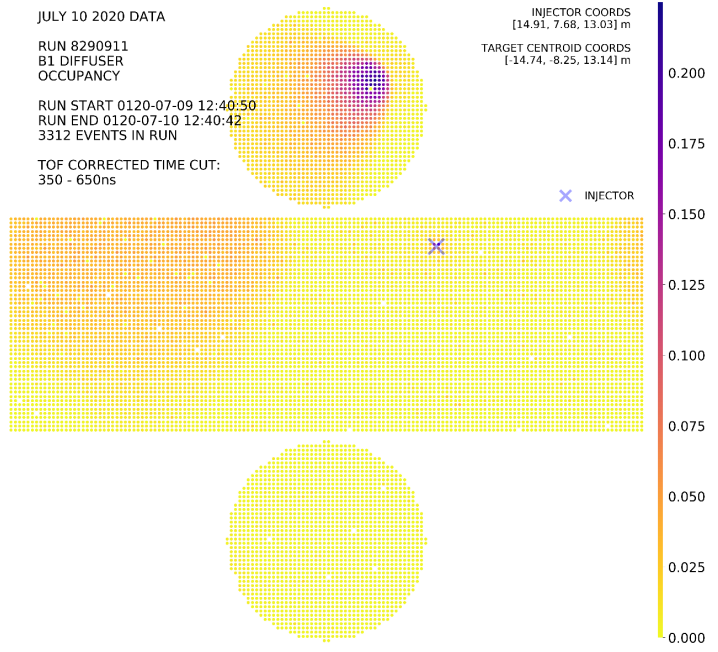
\includegraphics[width=0.49\textwidth]{Figures/B1_occupancy_diff_auto.PNG}} \hfill
    \subfloat[B2 diffuser]{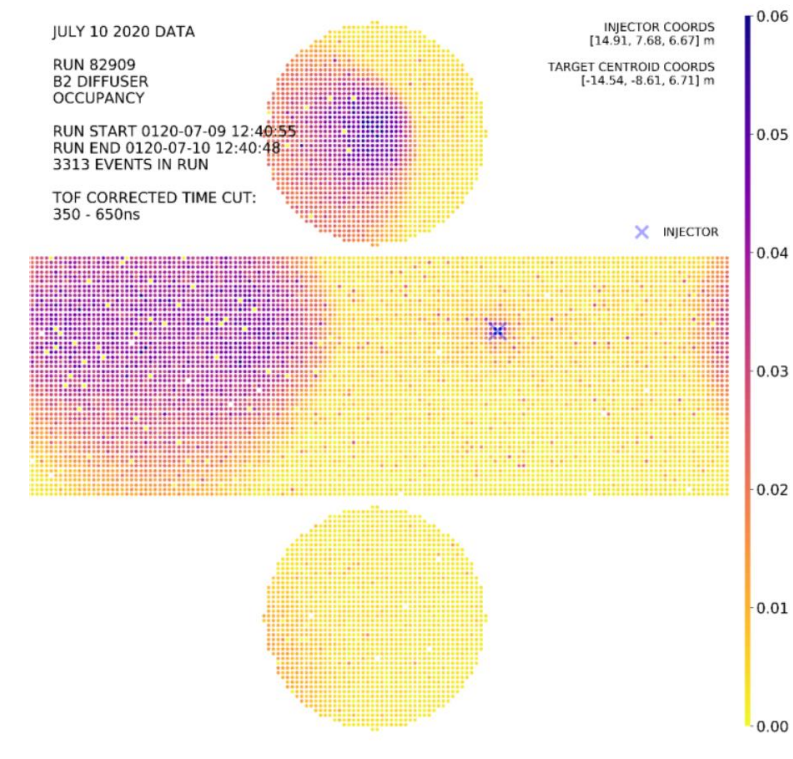
\includegraphics[width=0.49\textwidth]{Figures/B2_occupancy_diff_auto.PNG}} \par
    \subfloat[B3 diffuser]{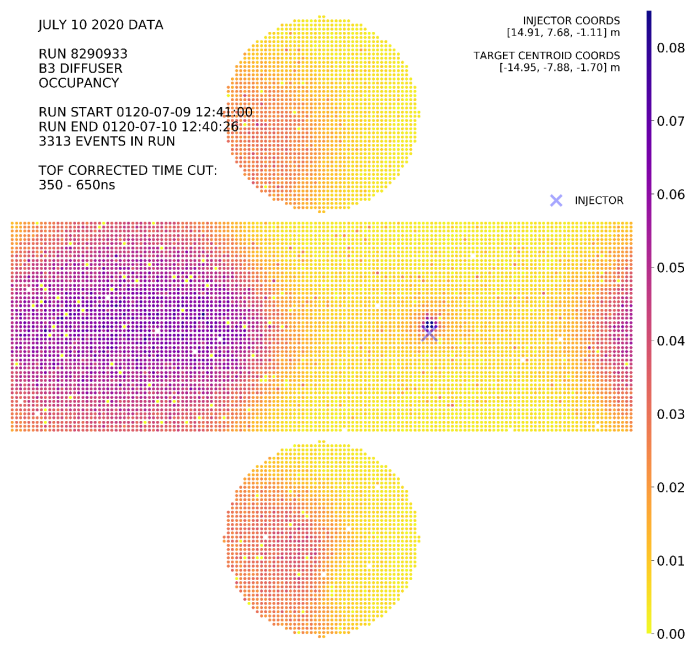
\includegraphics[width=0.49\textwidth]{Figures/B3_occupancy_diff_auto.PNG}} \hfill
    \subfloat[B4 diffuser]{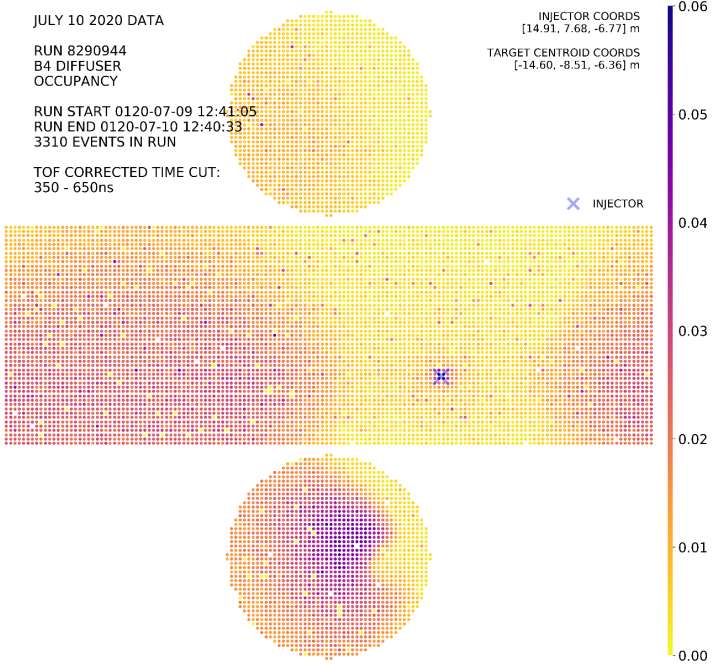
\includegraphics[width=0.49\textwidth]{Figures/B4_occupancy_diff_auto.PNG}} \par
    \subfloat[B5 diffuser]{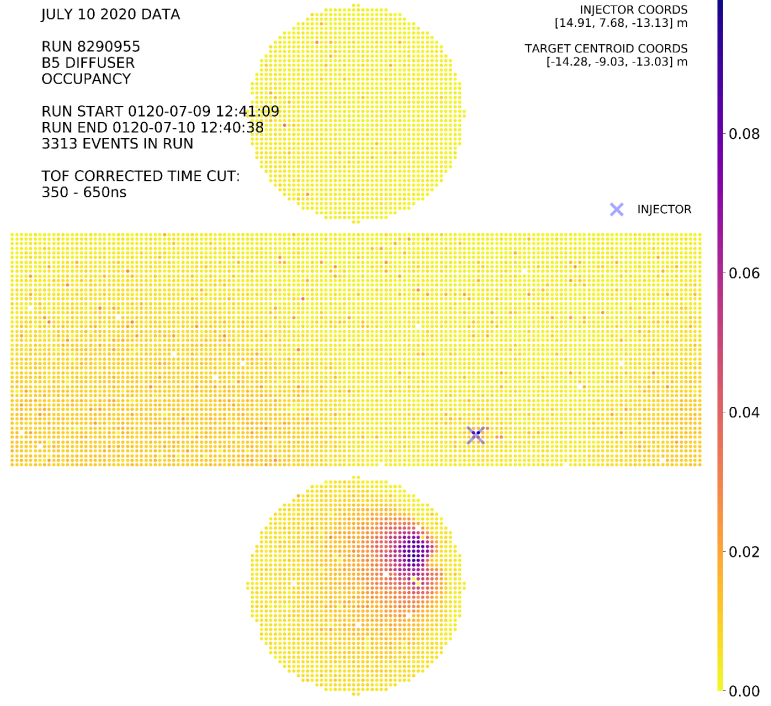
\includegraphics[width=0.49\textwidth]{Figures/B5_occupancy_diff_auto.PNG}}
    
\end{figure}

\begin{figure}
    \centering
    
    \caption{Occupancy plot for the diffuser optics from the UKLI Autocalib July 2020 run} \label{fig:occupancy_diff_auto} 
    
    \subfloat[B1 diffuser]{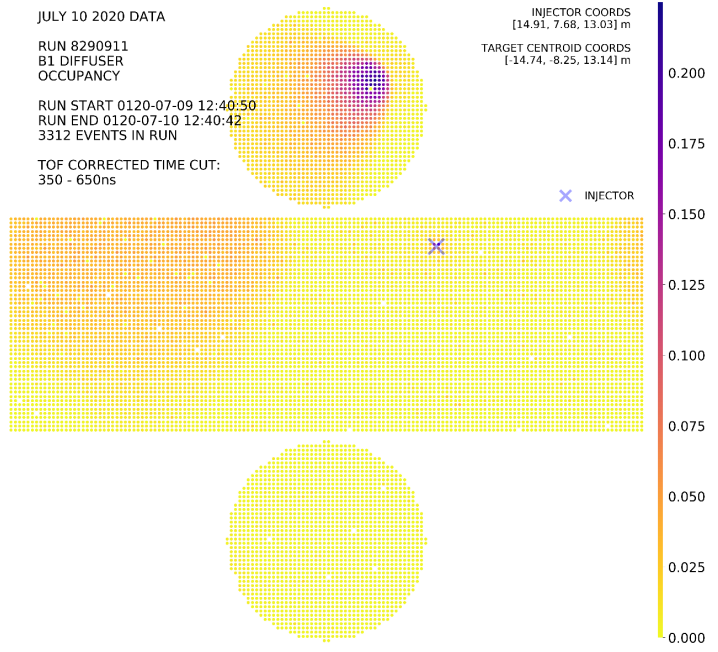
\includegraphics[width=0.49\textwidth]{Figures/B1_occupancy_diff_auto.PNG}} \hfill
    \subfloat[B2 diffuser]{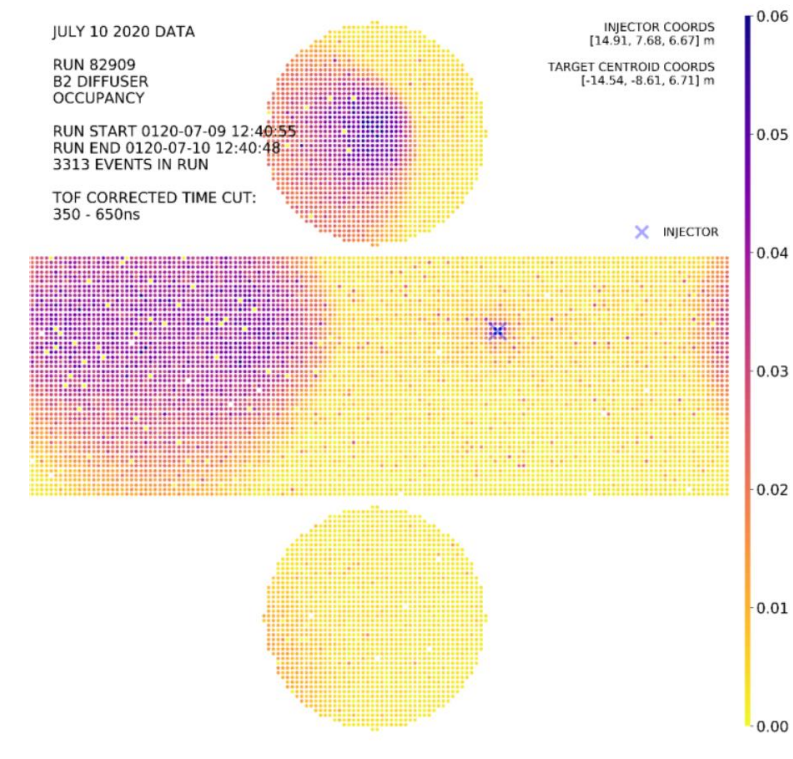
\includegraphics[width=0.49\textwidth]{Figures/B2_occupancy_diff_auto.PNG}} \par
    \subfloat[B3 diffuser]{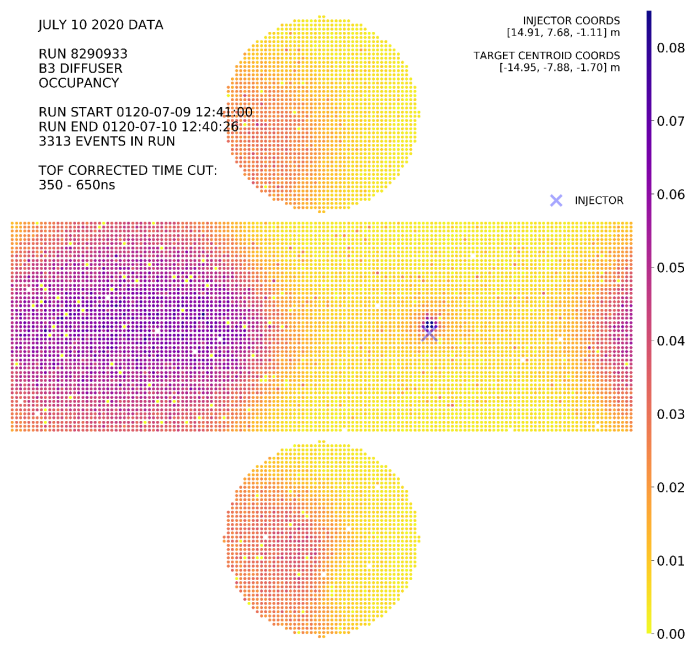
\includegraphics[width=0.49\textwidth]{Figures/B3_occupancy_diff_auto.PNG}} \hfill
    \subfloat[B4 diffuser]{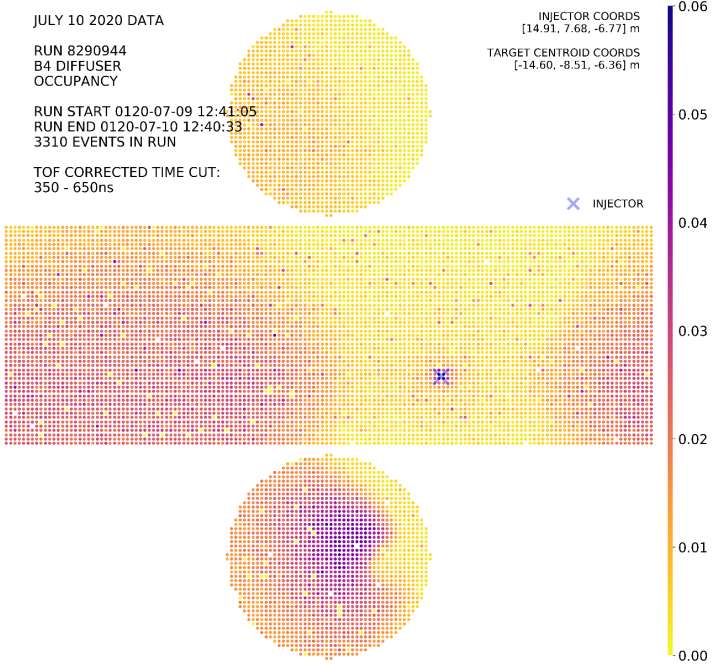
\includegraphics[width=0.49\textwidth]{Figures/B4_occupancy_diff_auto.PNG}} \par
    \subfloat[B5 diffuser]{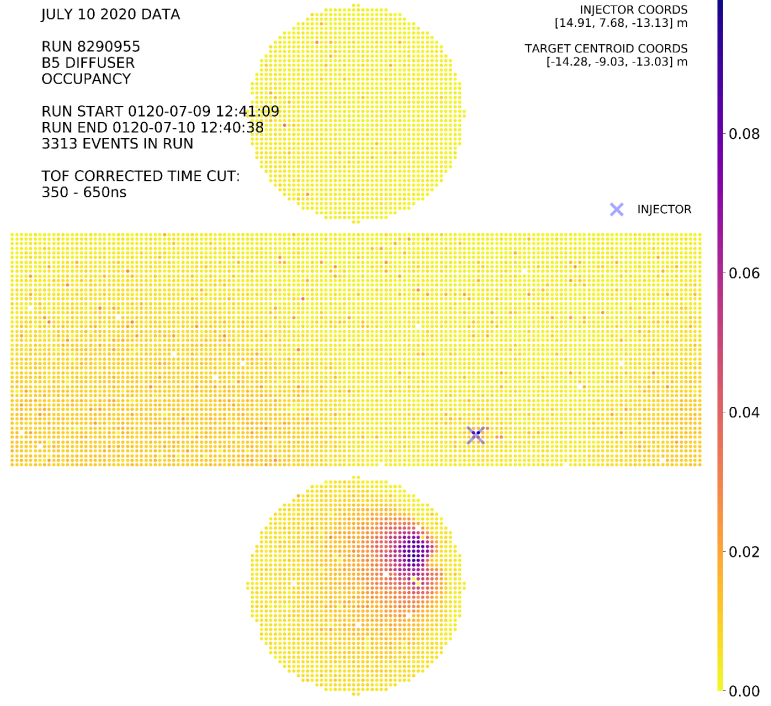
\includegraphics[width=0.49\textwidth]{Figures/B5_occupancy_diff_auto.PNG}}
    
\end{figure}

\begin{figure}
    \centering
    
    \caption{Occupancy plot for the collimator optics from the UKLI Autocalib July 2020 run} \label{fig:occupancy_coll_auto} 
    
    \subfloat[B1 collimator]{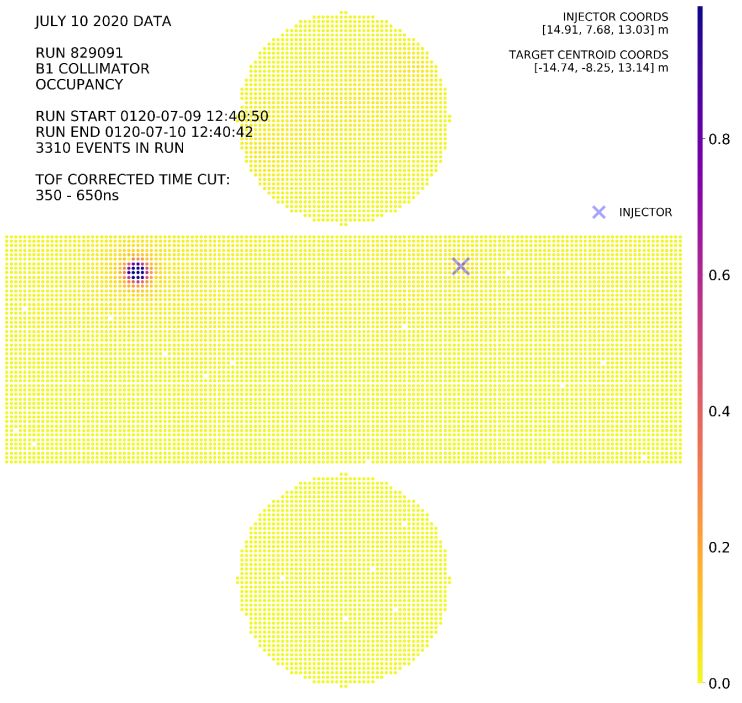
\includegraphics[width=0.49\textwidth]{Figures/B1_occupancy_coll_auto.PNG}} \hfill
    \subfloat[B2 collimator]{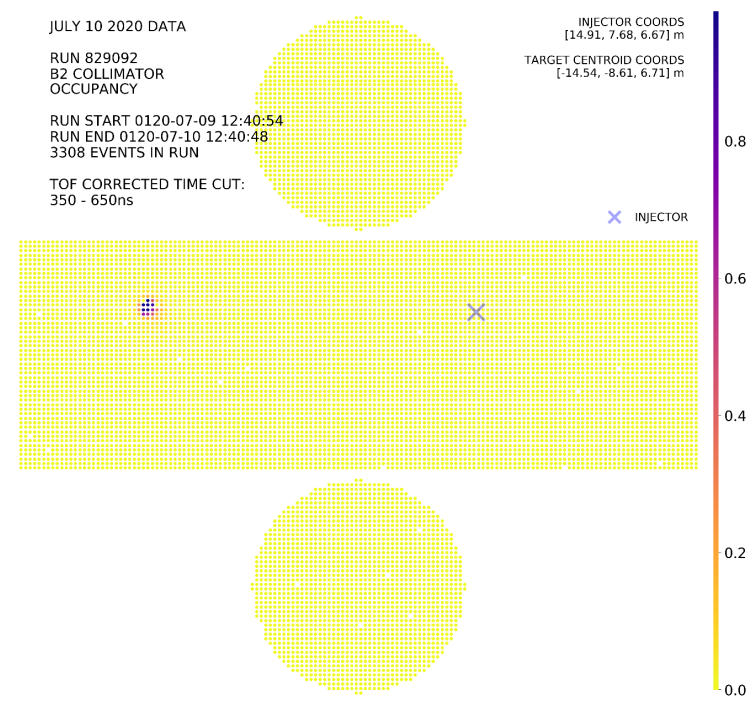
\includegraphics[width=0.49\textwidth]{Figures/B2_occupancy_coll_auto.PNG}} \par
    \subfloat[B3 collimator]{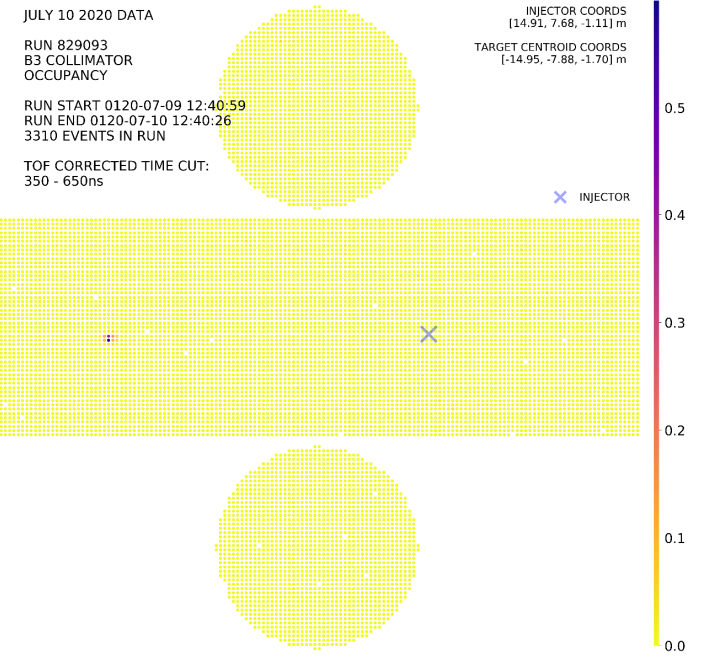
\includegraphics[width=0.49\textwidth]{Figures/B3_occupancy_coll_auto.PNG}} \hfill
    \subfloat[B4 collimator]{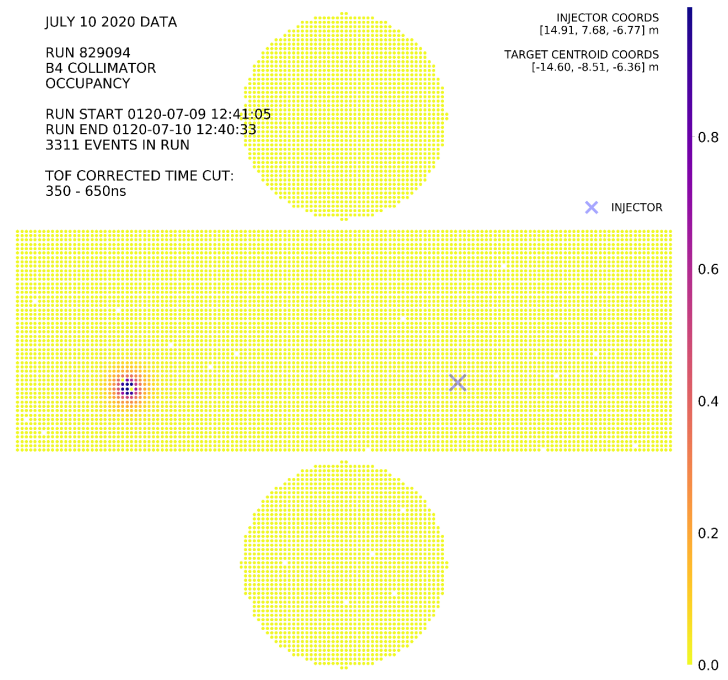
\includegraphics[width=0.49\textwidth]{Figures/B4_occupancy_coll_auto.PNG}} \par
    \subfloat[B5 collimator]{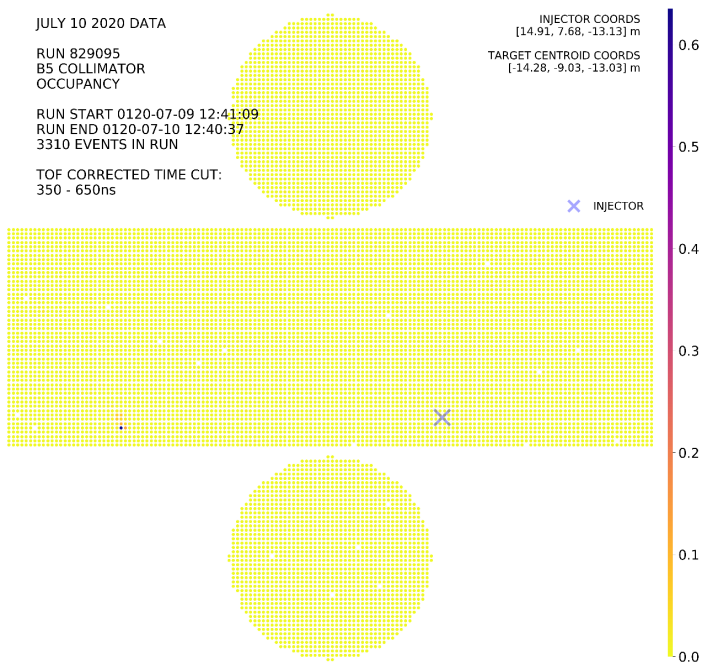
\includegraphics[width=0.49\textwidth]{Figures/B5_occupancy_coll_auto.PNG}}
    
\end{figure}

\begin{figure}
    \centering
    
    \caption{Occupancy plot for the diffuser optics from the UKLI Autocalib July 2020 run} \label{fig:occupancy_diff_auto} 
    
    \subfloat[B1 diffuser]{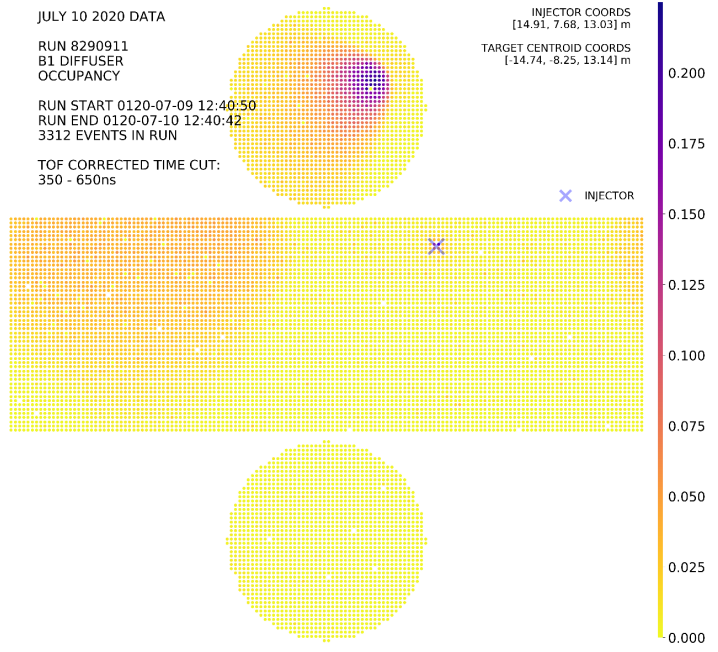
\includegraphics[width=0.49\textwidth]{Figures/B1_occupancy_diff_auto.PNG}} \hfill
    \subfloat[B2 diffuser]{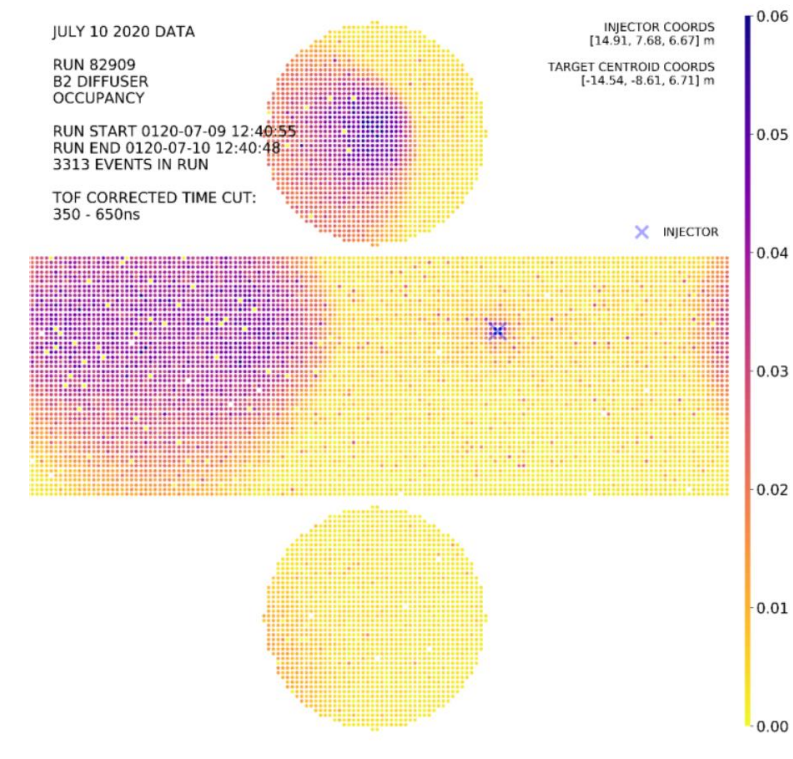
\includegraphics[width=0.49\textwidth]{Figures/B2_occupancy_diff_auto.PNG}} \par
    \subfloat[B3 diffuser]{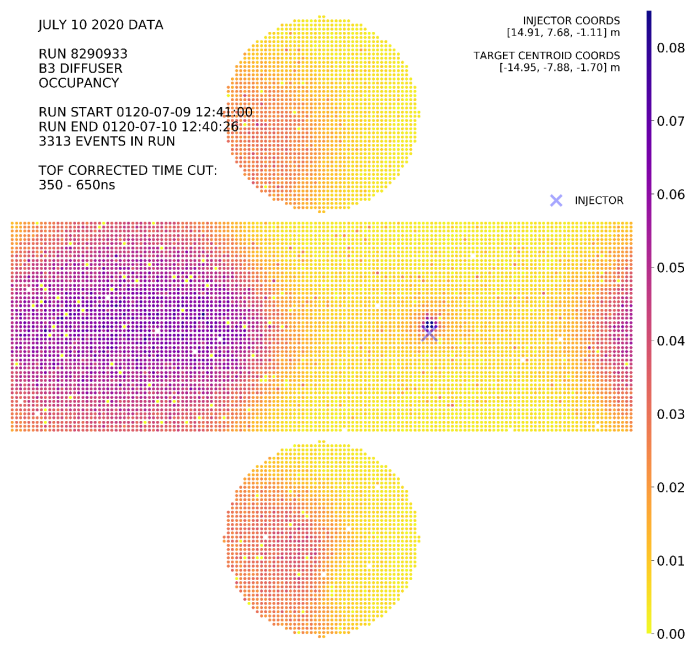
\includegraphics[width=0.49\textwidth]{Figures/B3_occupancy_diff_auto.PNG}} \hfill
    \subfloat[B4 diffuser]{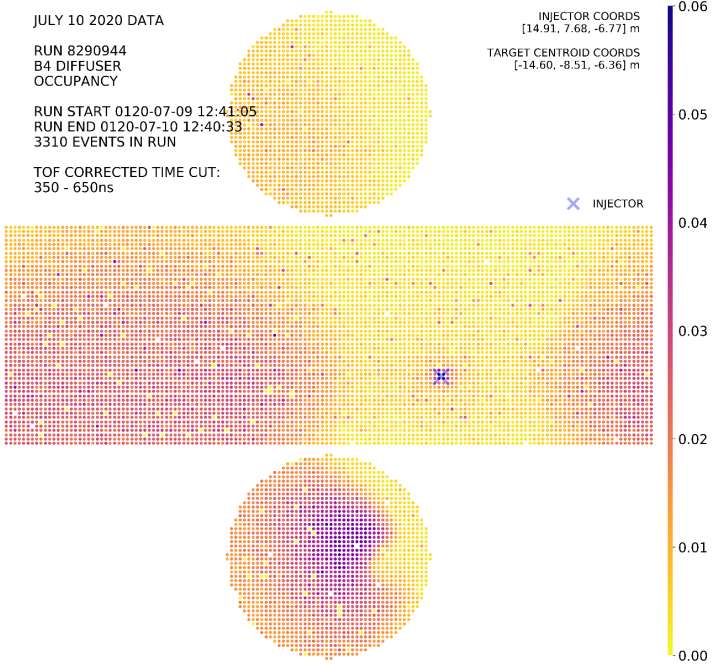
\includegraphics[width=0.49\textwidth]{Figures/B4_occupancy_diff_auto.PNG}} \par
    \subfloat[B5 diffuser]{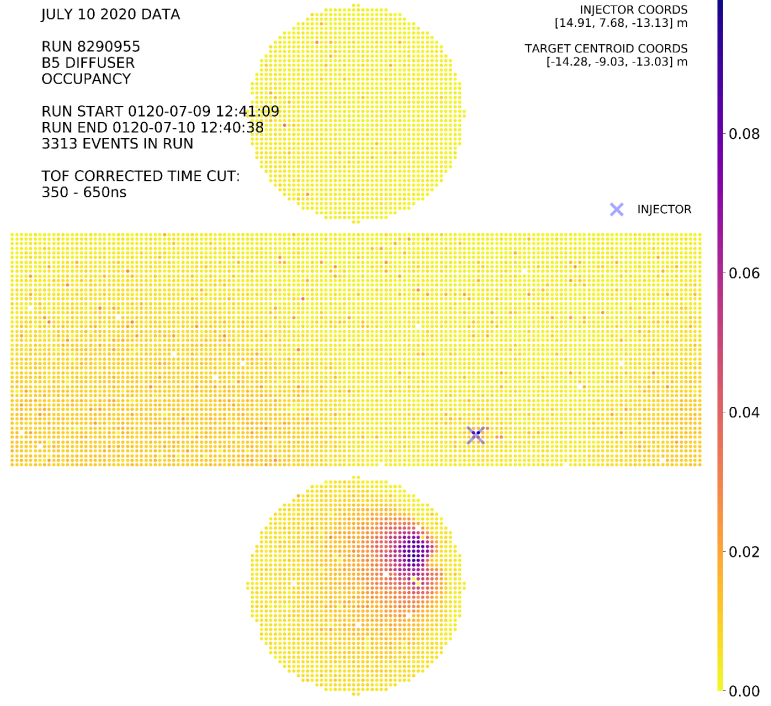
\includegraphics[width=0.49\textwidth]{Figures/B5_occupancy_diff_auto.PNG}}
    
\end{figure}


Figure \ref{fig:PDF_CDF_coll} shows the complete PDFs and CDFs for the B1 - B5 collimator data taken from the test stand at Warwick and Figure \ref{fig:PDF_CDF_diff} shows the complete PDFs and CDFs for the B1 - B5 diffusers. Figure \ref{fig:PDF_CDF_inv_coll} show the inverse CDF fits for the collimator, and Figure \ref{fig:PDF_CDF_inv_diff} shows the inverse CDF fits for the diffuser. 

\begin{figure}[!htbp]
    \centering
    
    \caption{PDFs and corresponding CDFs for the B1 - B5 collimators} 
    \label{fig:PDF_CDF_coll}
    \subfloat[B1 collimator PDF]{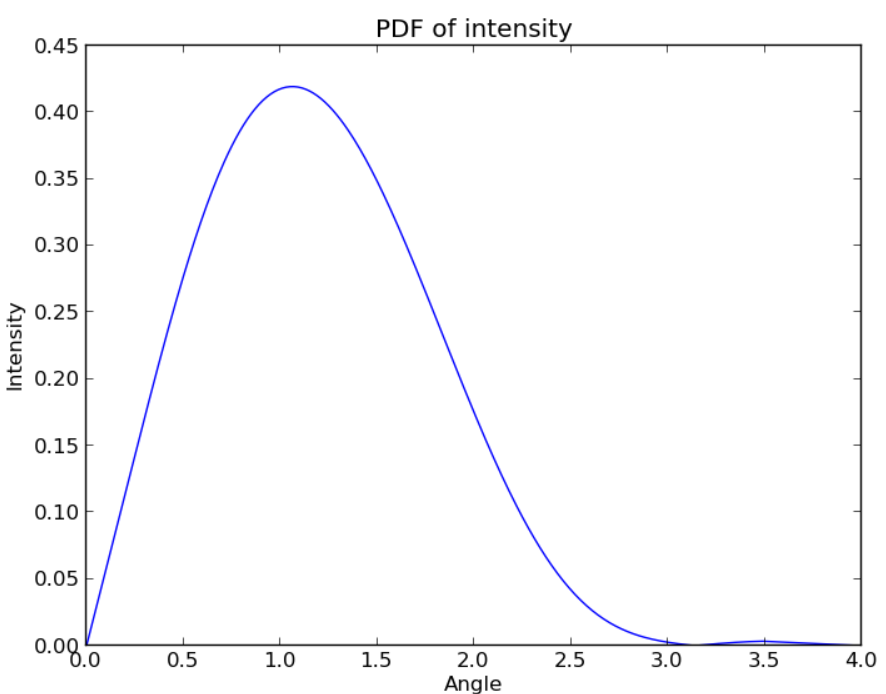
\includegraphics[width=0.49\textwidth]{Figures/B1_coll_pdf.png}}\hfill
    \subfloat[B1 collimator CDF]{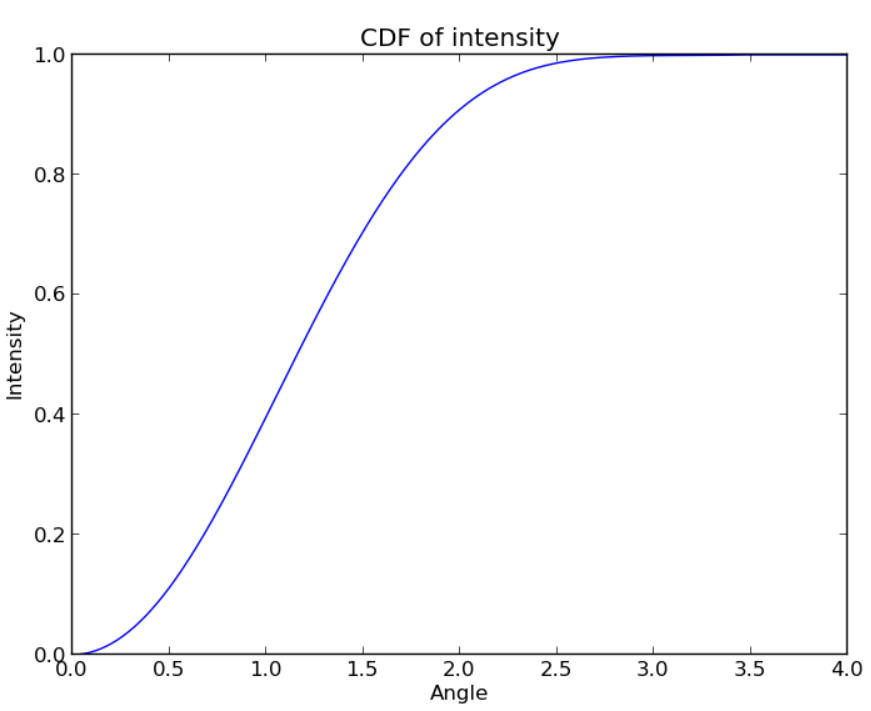
\includegraphics[width=0.49\textwidth]{Figures/B1_coll_cdf.png}} \par
    \subfloat[B2 collimator PDF]{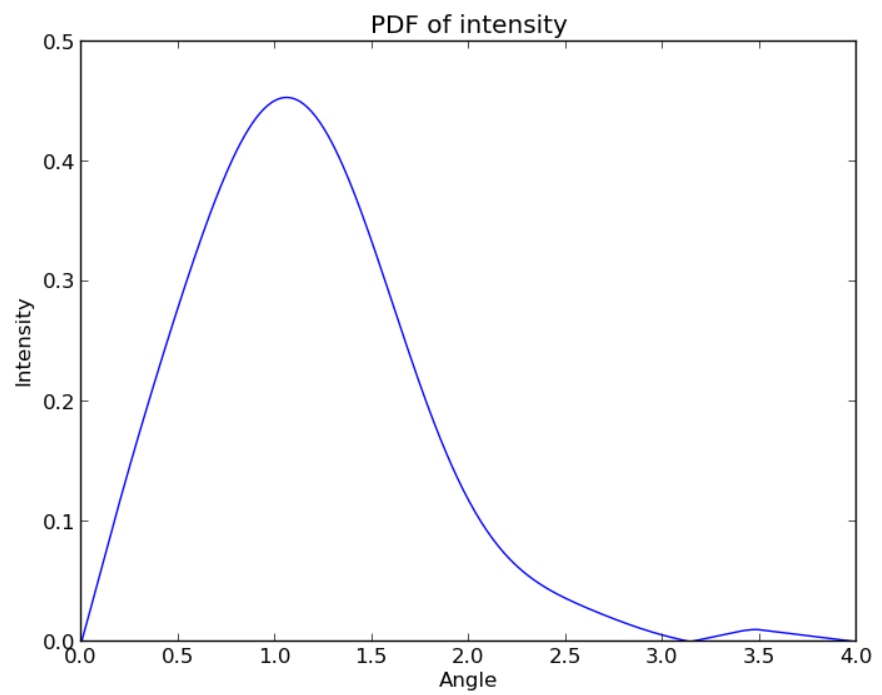
\includegraphics[width=0.49\textwidth]{Figures/B2_coll_pdf.png}} \hfill
    \subfloat[B2 collimator CDF]{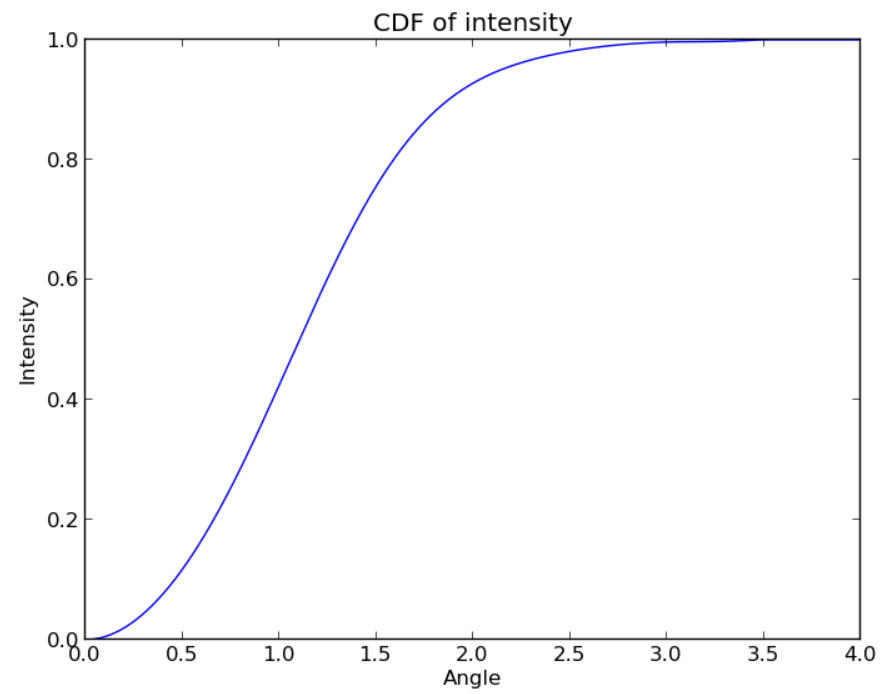
\includegraphics[width=0.49\textwidth]{Figures/B2_coll_cdf.png}} \par
    \subfloat[B3 collimator PDF]{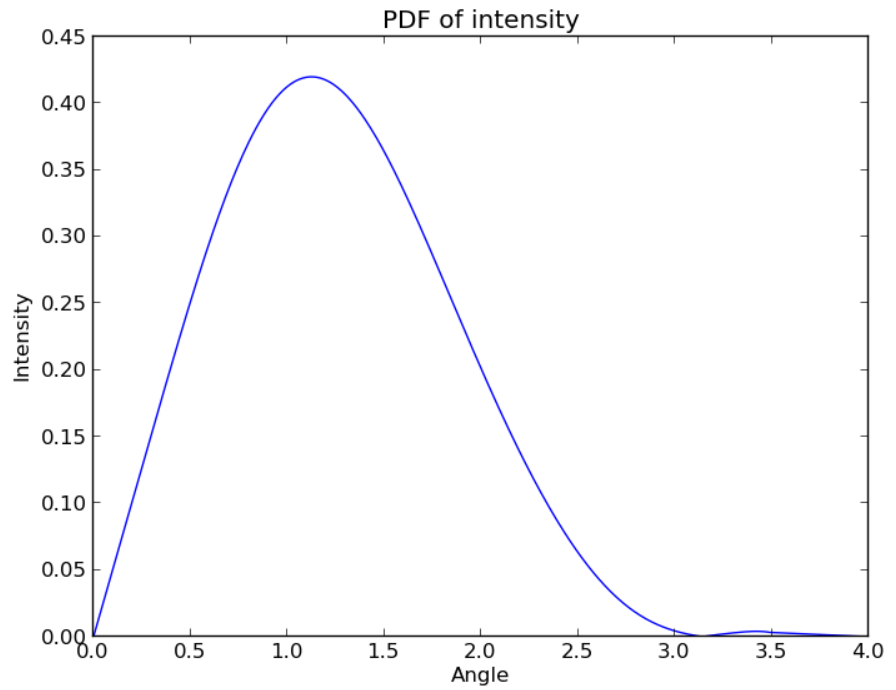
\includegraphics[width=0.49\textwidth]{Figures/B3_coll_pdf.png}} \hfill
    \subfloat[B3 collimator CDF]{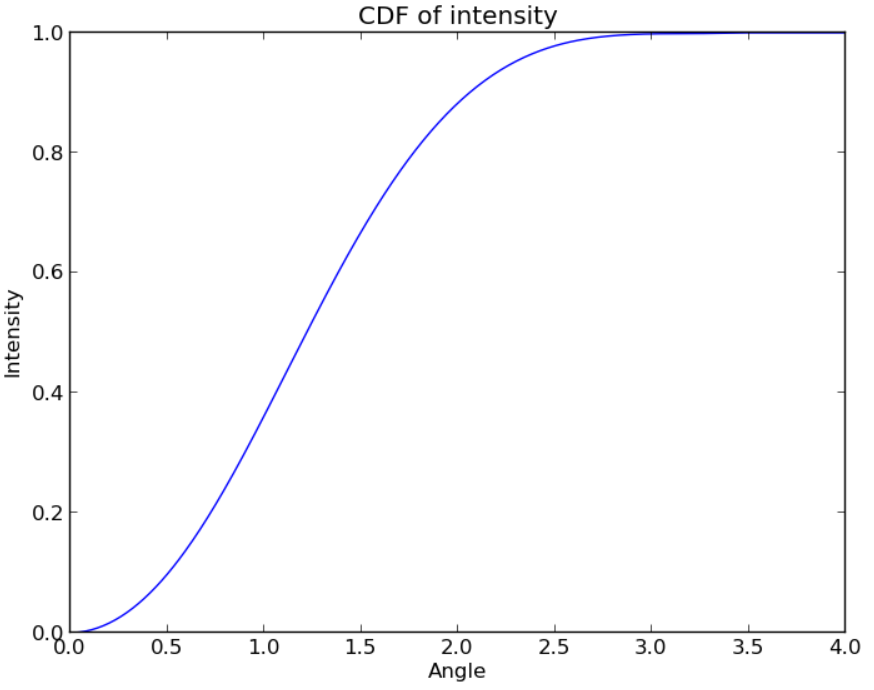
\includegraphics[width=0.49\textwidth]{Figures/B3_coll_cdf.png}} \par 
\end{figure}
\begin{figure}[!htbp]
    \ContinuedFloat
    \subfloat[B4 collimator PDF]{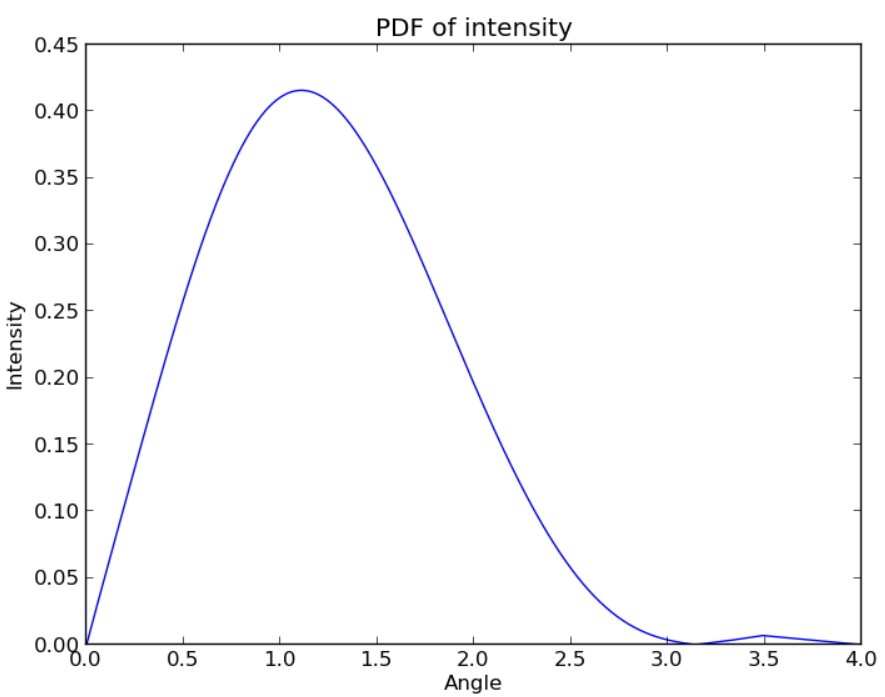
\includegraphics[width=0.49\textwidth]{Figures/B4_coll_pdf.png}} \hfill
    \subfloat[B4 collimator CDF]{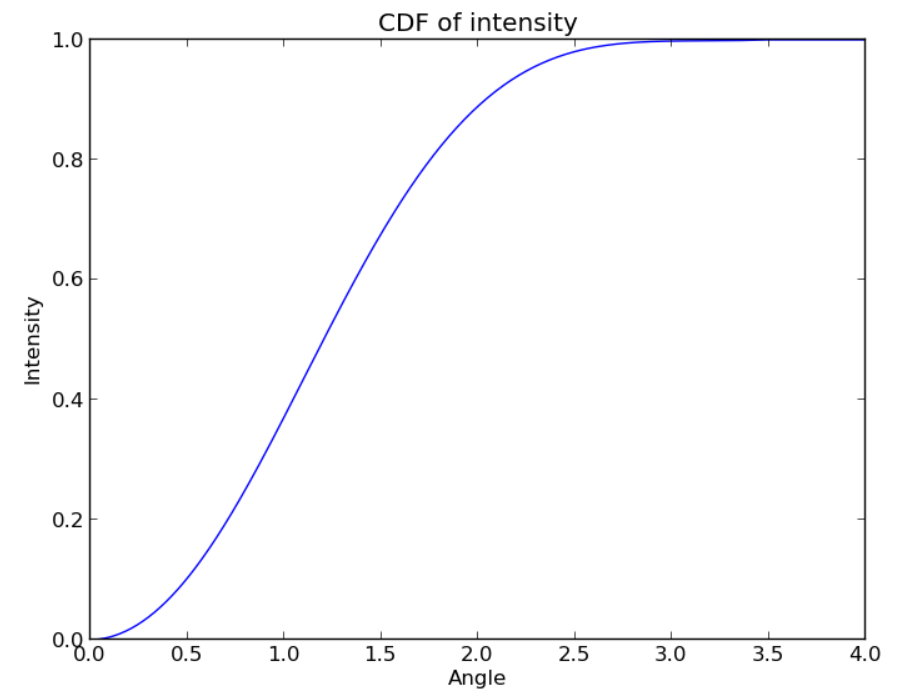
\includegraphics[width=0.49\textwidth]{Figures/B4_coll_cdf.png}} \par
    \subfloat[B5 collimator PDF]{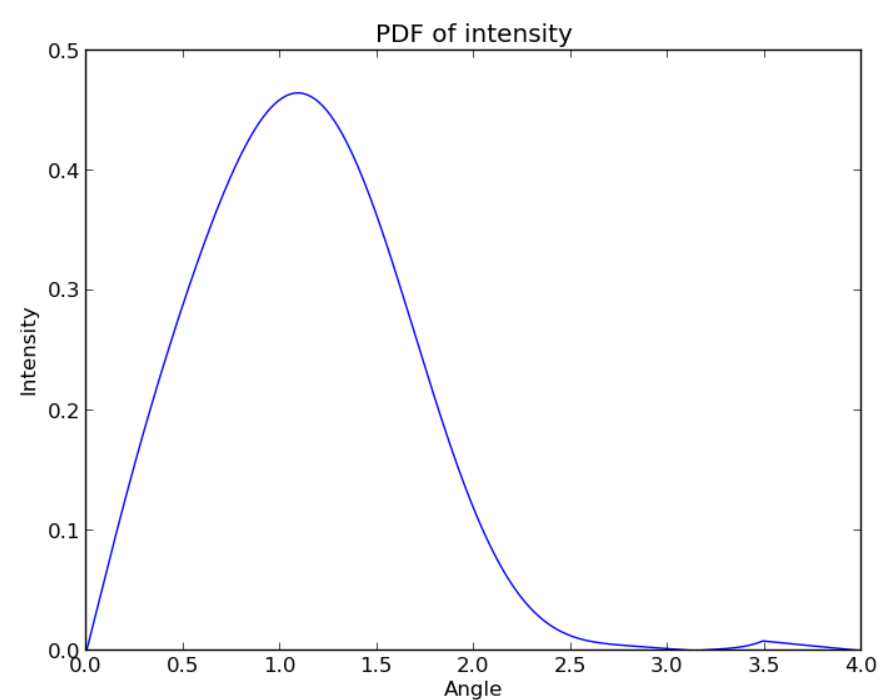
\includegraphics[width=0.49\textwidth]{Figures/B5_coll_pdf.png}} \hfill
    \subfloat[B5 collimator CDF]{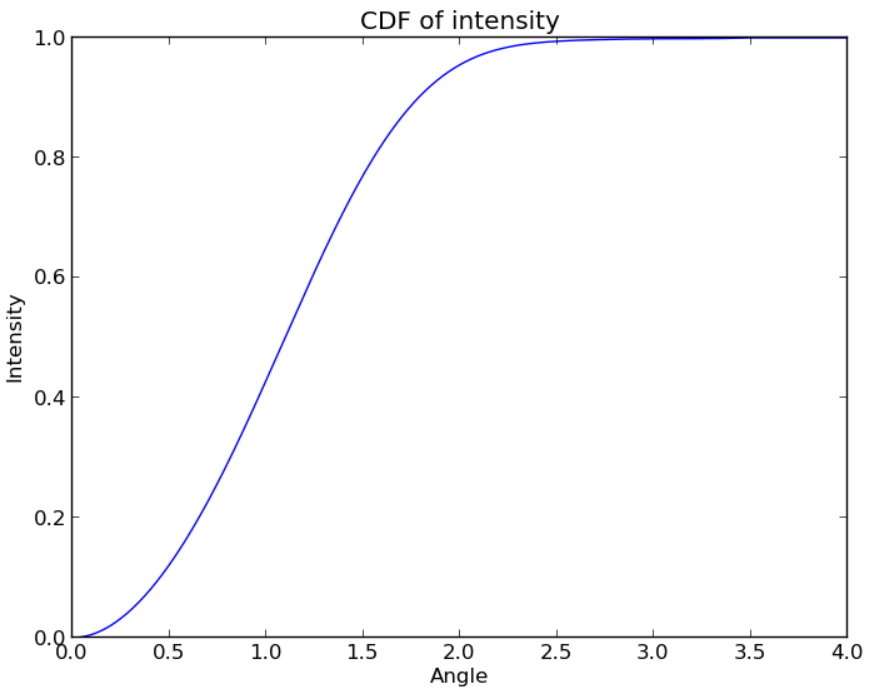
\includegraphics[width=0.49\textwidth]{Figures/B5_coll_cdf.png} } 
    
    
\end{figure}

\begin{figure}[!htbp]
    \centering
    
    \caption{PDFs and corresponding CDFs for the B1 - B5 diffusers} 
    \label{fig:PDF_CDF_diff}
    \subfloat[B1 diffuser PDF]{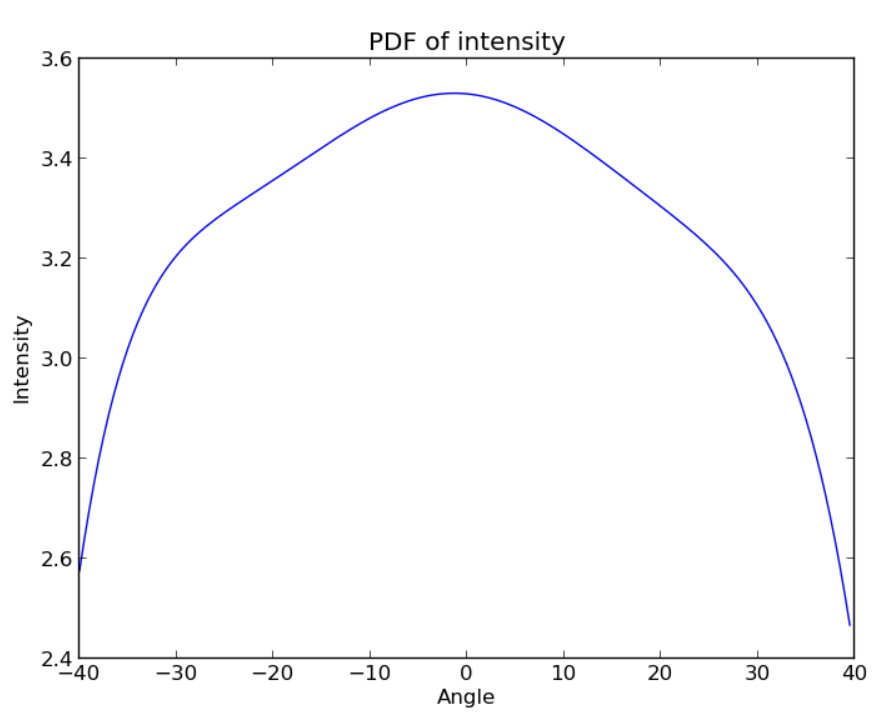
\includegraphics[width=0.49\textwidth]{Figures/B1_diff_pdf.png}} \hfill
    \subfloat[B1 diffuser CDF]{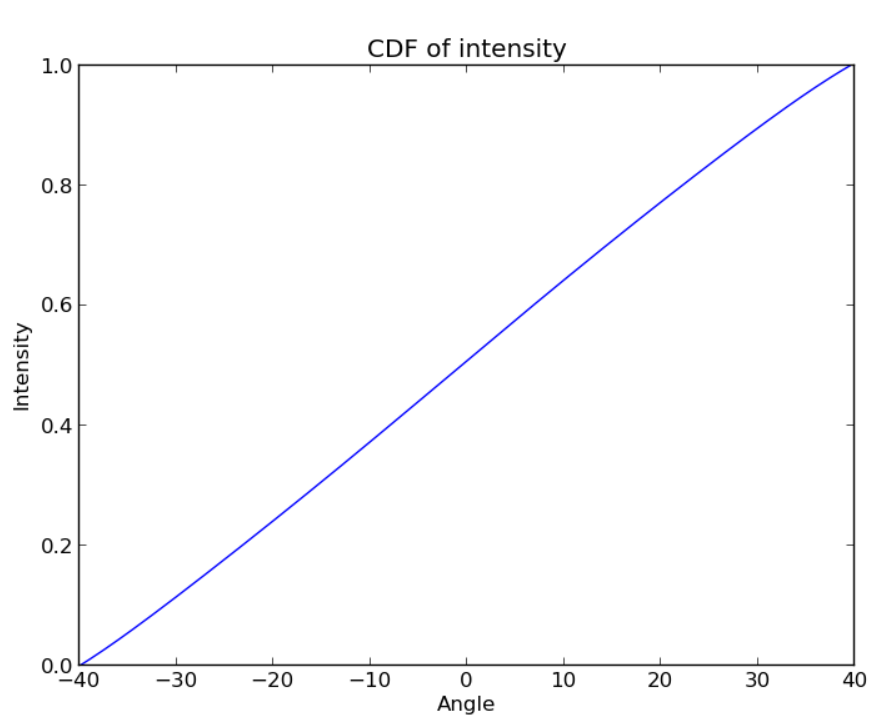
\includegraphics[width=0.49\textwidth]{Figures/B1_diff_cdf.png}} \par
    \subfloat[B2 diffuser PDF]{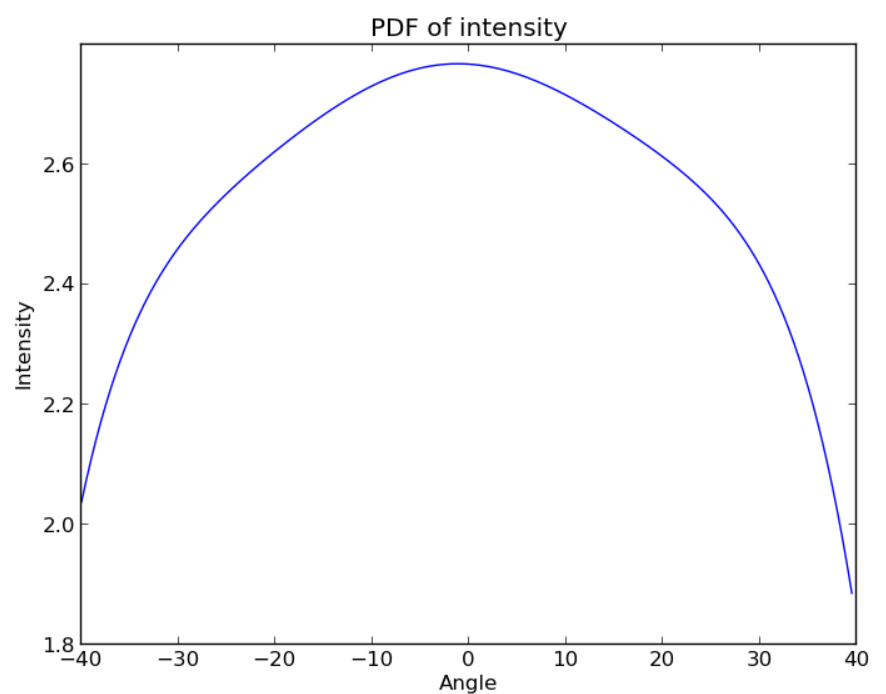
\includegraphics[width=0.49\textwidth]{Figures/B2_diff_pdf.png}} \hfill
    \subfloat[B2 diffuser CDF]{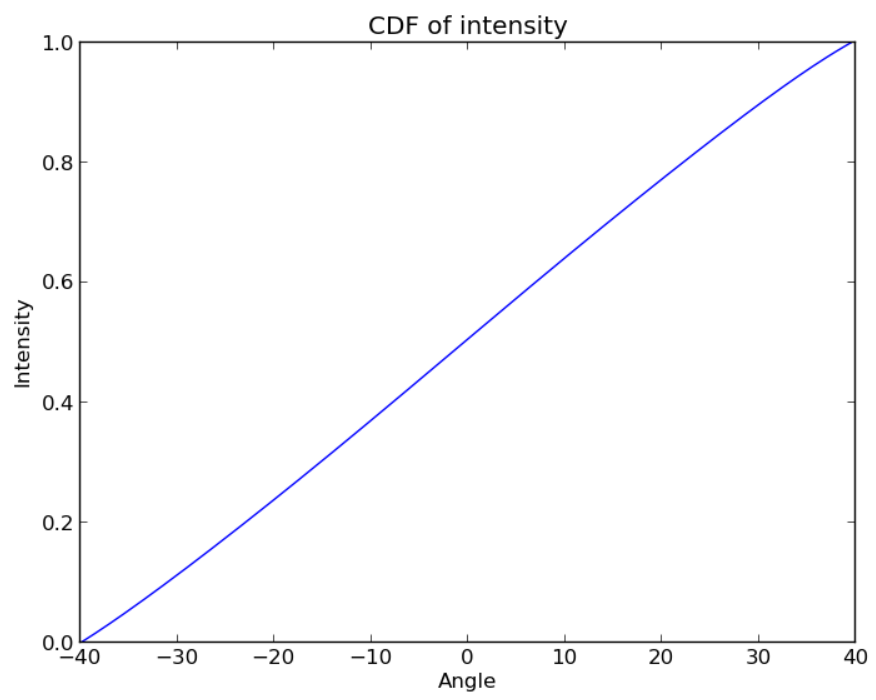
\includegraphics[width=0.49\textwidth]{Figures/B2_diff_cdf.png}} \par
    \subfloat[B3 diffuser PDF]{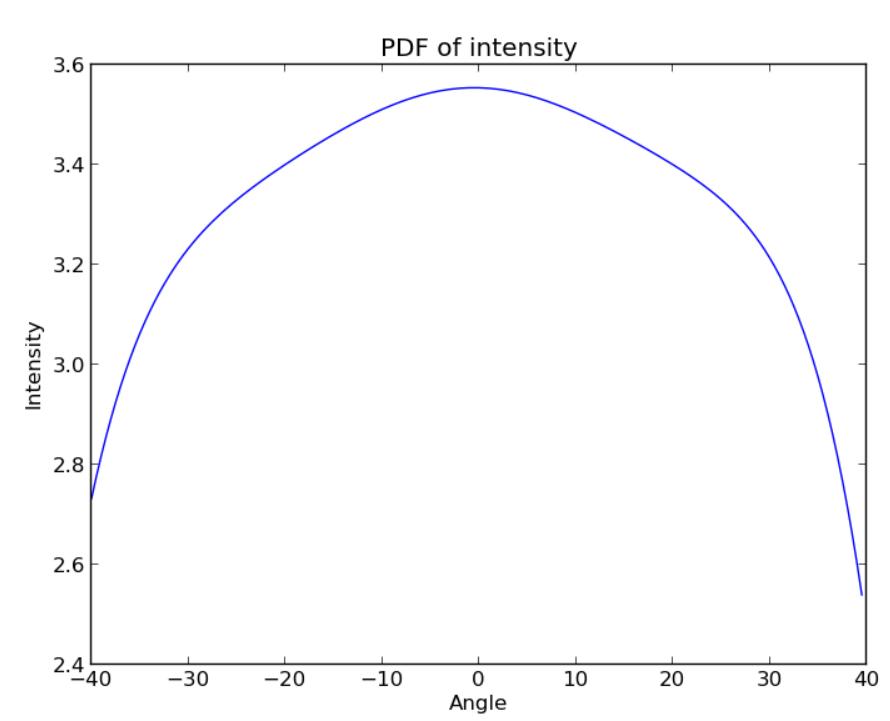
\includegraphics[width=0.49\textwidth]{Figures/B3_diff_pdf.png}} \hfill
    \subfloat[B3 diffuser CDF]{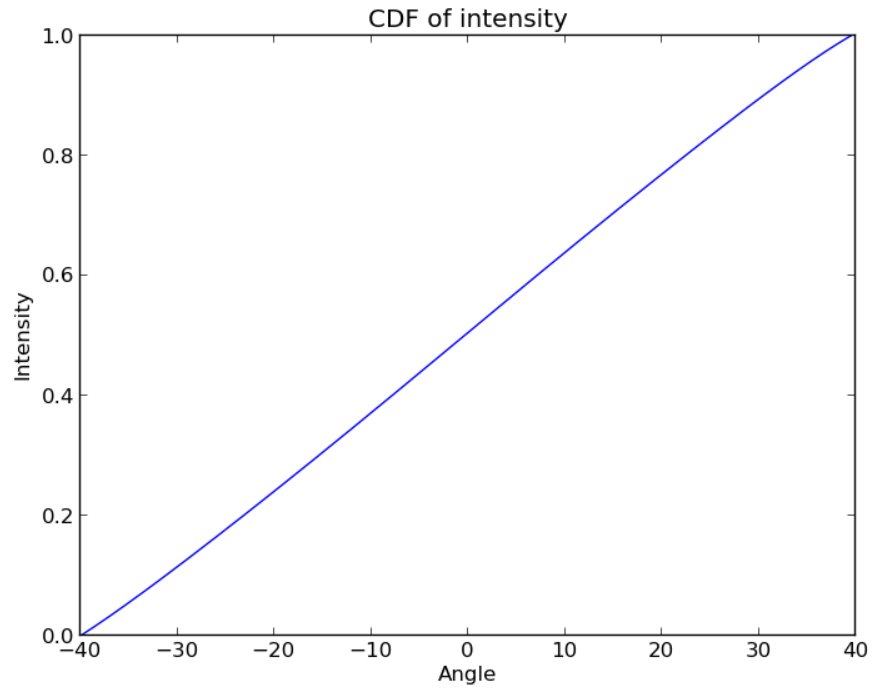
\includegraphics[width=0.49\textwidth]{Figures/B3_diff_cdf.png}} 
\end{figure}
\begin{figure}[!htbp]
    \ContinuedFloat
    \subfloat[B4 diffuser PDF]{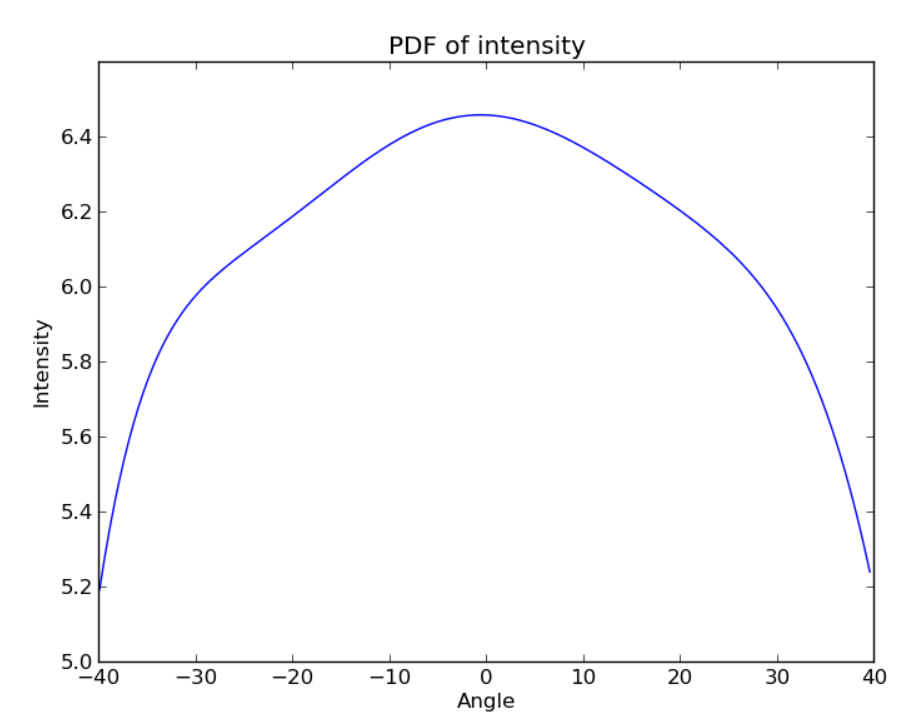
\includegraphics[width=0.49\textwidth]{Figures/B4_diff_pdf.png}} \hfill
    \subfloat[B4 diffuser CDF]{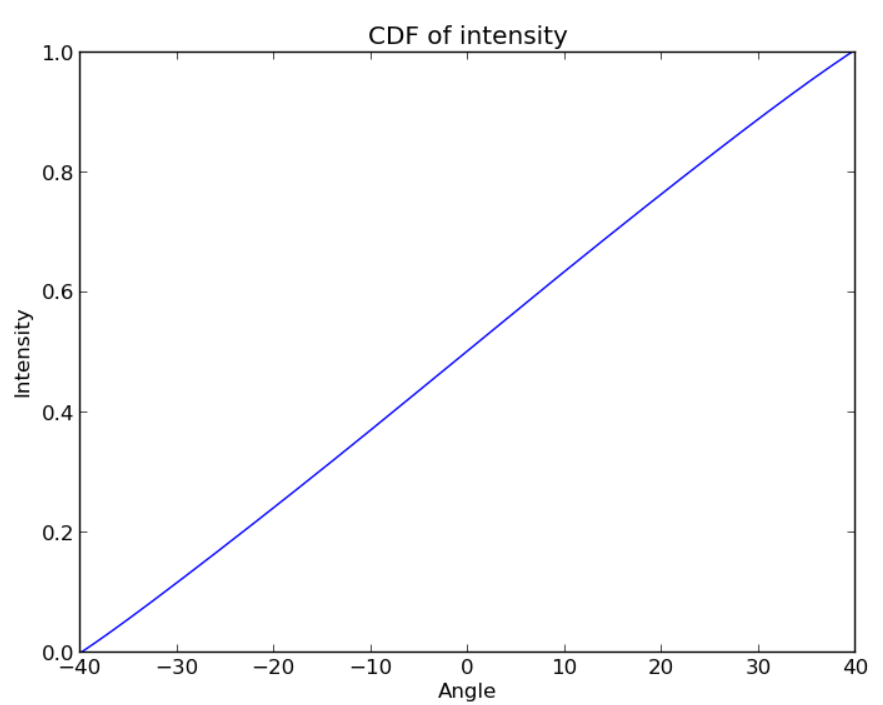
\includegraphics[width=0.49\textwidth]{Figures/B4_diff_cdf.png}} \par
    \subfloat[B5 diffuser PDF]{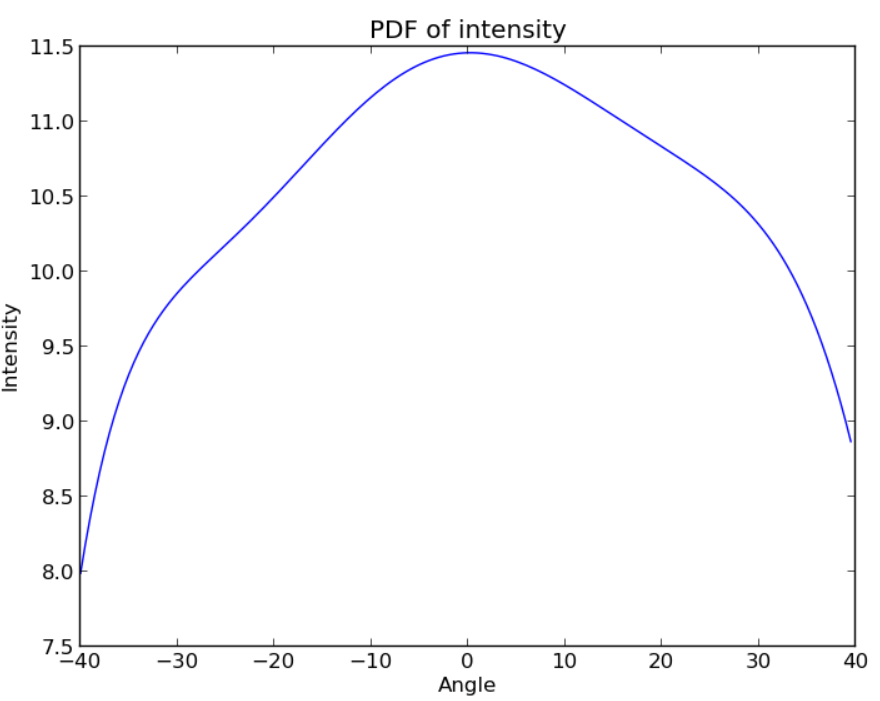
\includegraphics[width=0.49\textwidth]{Figures/B5_diff_pdf.png}} \hfill
    \subfloat[B5 diffuser CDF]{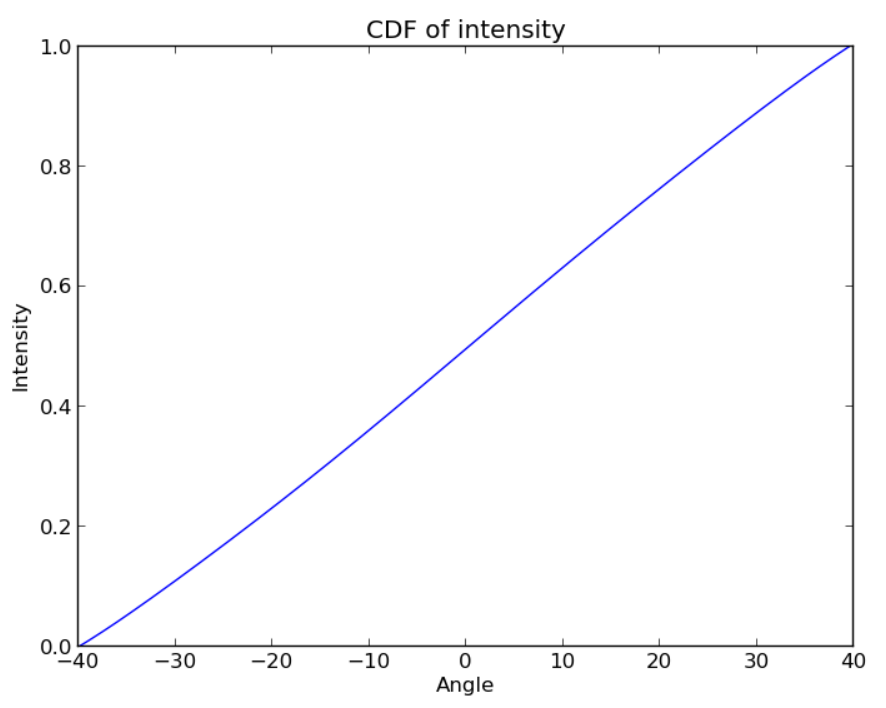
\includegraphics[width=0.49\textwidth]{Figures/B5_diff_cdf.png}}      
\end{figure}

\begin{figure}[!htbp]
    \centering
        
    \caption{CDF and inverse CDF fits for the B1 - B5 collimator PDFs}  
    \label{fig:PDF_CDF_inv_coll}
        \subfloat[B1 inverse collimator CDF]{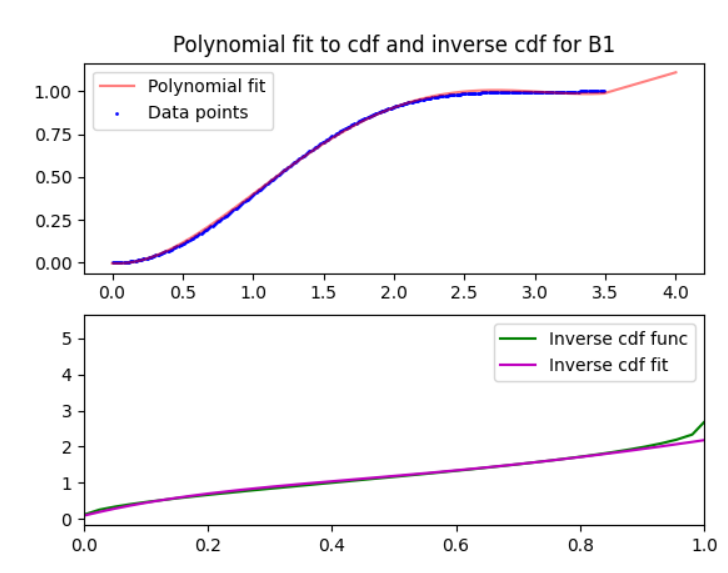
\includegraphics[width=0.49\textwidth]{Figures/B1_inv_coll_cdf.png}} \hfill
        \subfloat[B2 inverse collimator CDF]{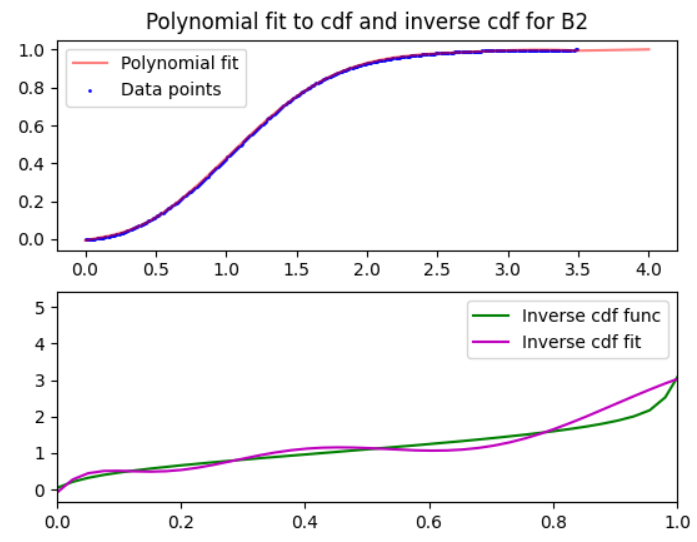
\includegraphics[width=0.49\textwidth]{Figures/B2_inv_coll_cdf.png}} \par
        \subfloat[B3 inverse collimator CDF]{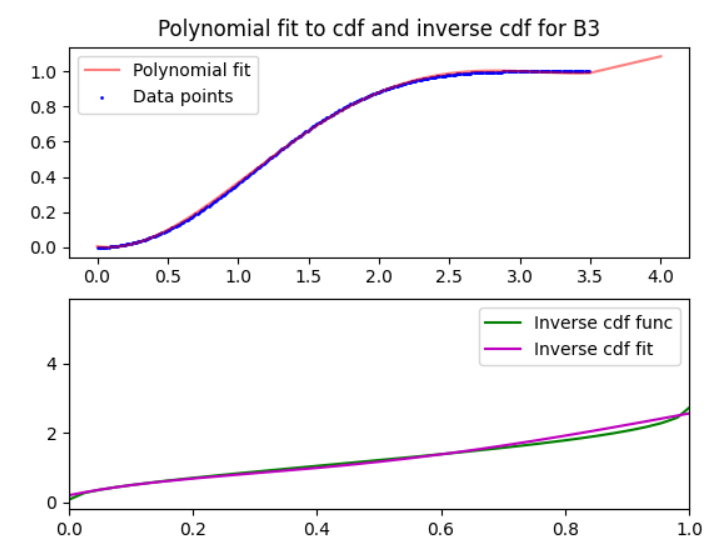
\includegraphics[width=0.49\textwidth]{Figures/B3_inv_coll_cdf.png}} \hfill
        \subfloat[B4 inverse collimator CDF]{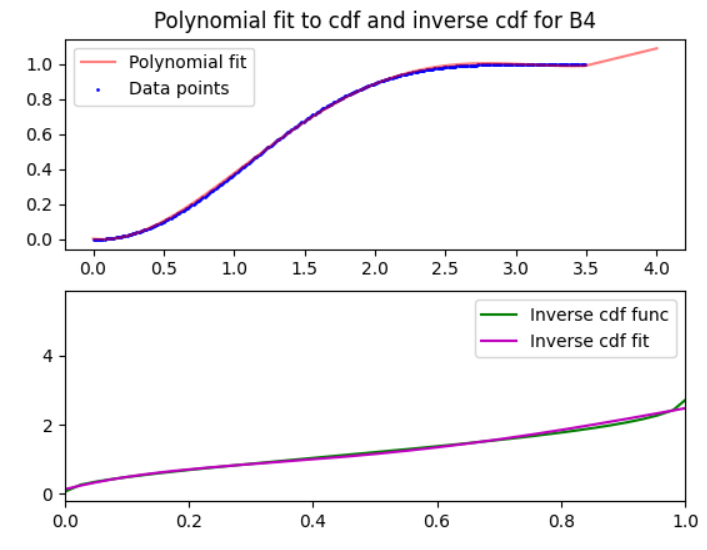
\includegraphics[width=0.49\textwidth]{Figures/B4_inv_coll_cdf.png}} \par
        \subfloat[B5 inverse collimator CDF]{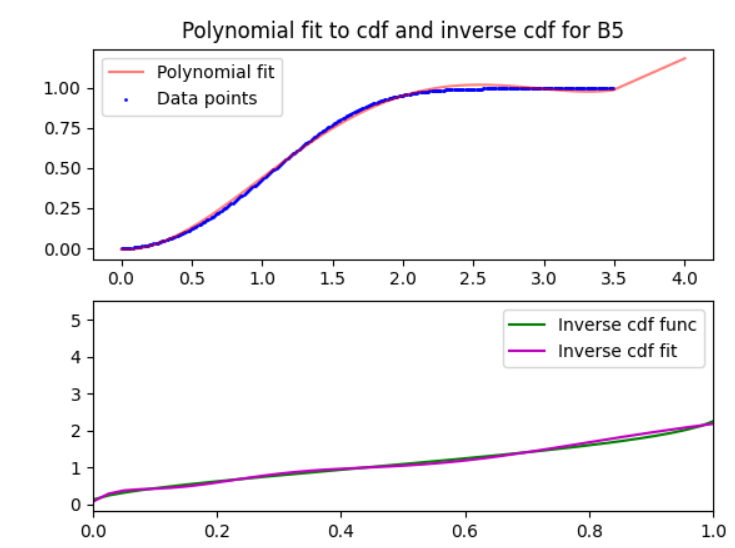
\includegraphics[width=0.49\textwidth]{Figures/B5_inv_coll_cdf.png}} 
    
    \end{figure}

    \begin{figure}[!htbp]
        \centering
            
        \caption{CDF and inverse CDF fits for the B1 - B5 diffuser PDFs}  
        \label{fig:PDF_CDF_inv_diff}   
            \subfloat[B1 inverse diffuser CDF]{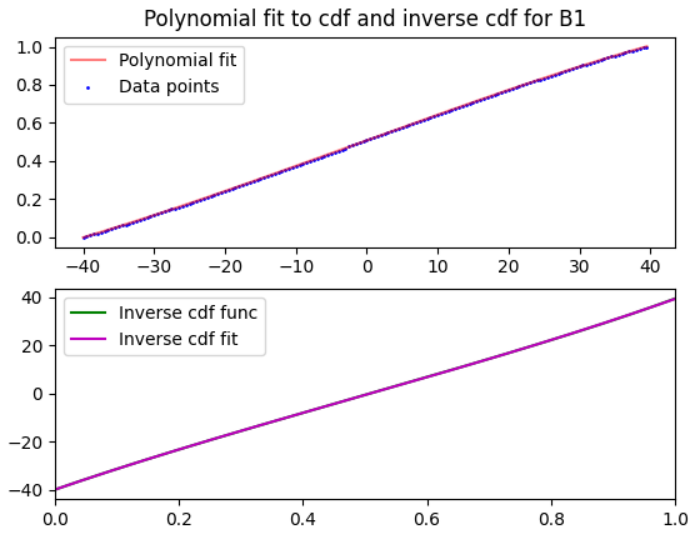
\includegraphics[width=0.49\textwidth]{Figures/B1_inv_diff_cdf.png}} \hfill
            \subfloat[B2 inverse diffuser CDF]{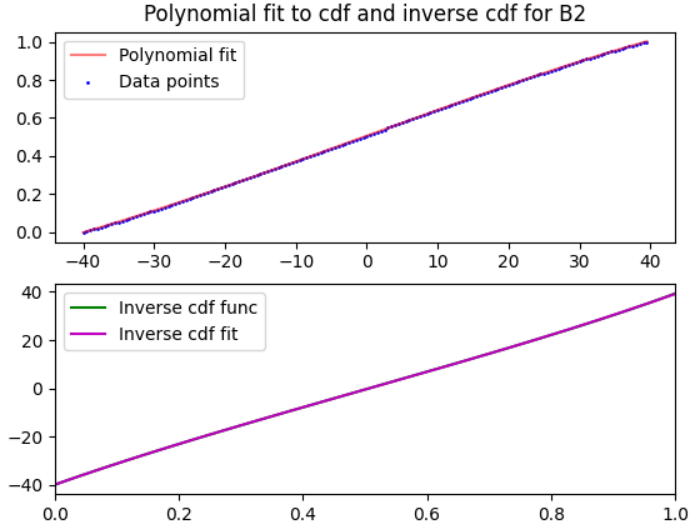
\includegraphics[width=0.49\textwidth]{Figures/B2_inv_diff_cdf.png}} \par
            \subfloat[B3 inverse diffuser CDF]{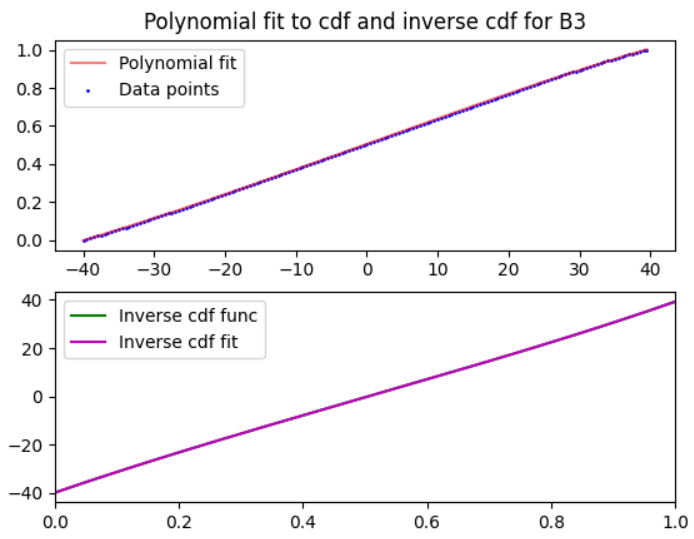
\includegraphics[width=0.49\textwidth]{Figures/B3_inv_diff_cdf.png}} \hfill
            \subfloat[B4 inverse diffuser CDF]{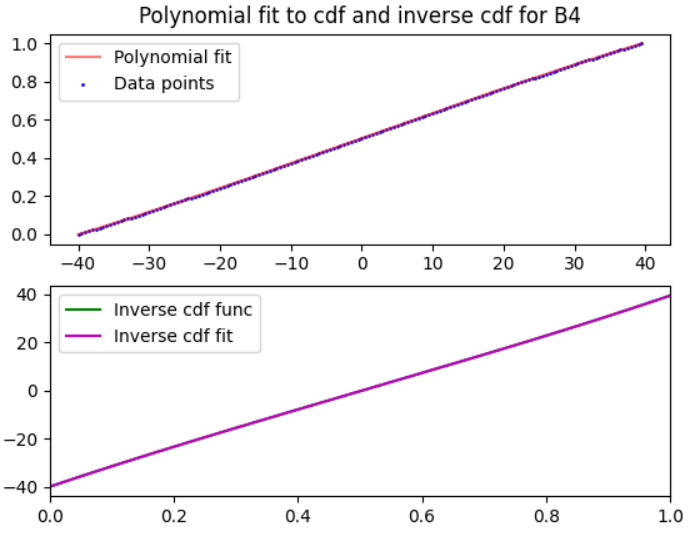
\includegraphics[width=0.49\textwidth]{Figures/B4_inv_diff_cdf.png}} \par
            \subfloat[B5 inverse diffuser CDF]{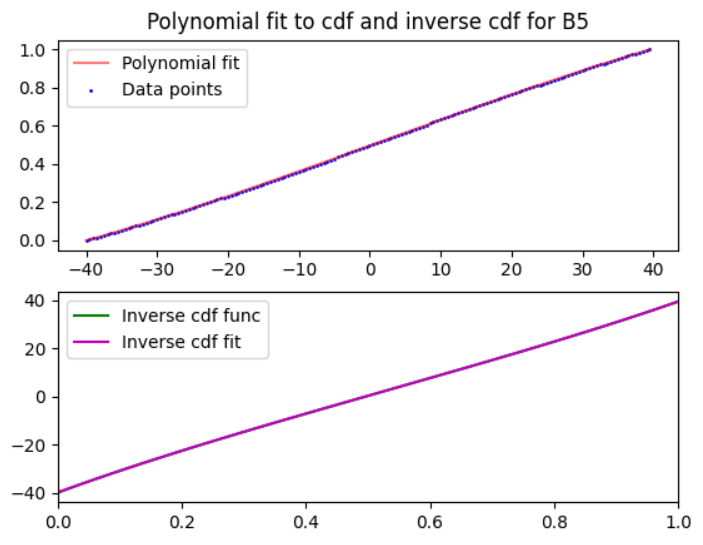
\includegraphics[width=0.49\textwidth]{Figures/B5_inv_diff_cdf.png}} 
        
    \end{figure}


    Figure \ref{fig:UKLI_MC_coll} shows the Monte Carlo simulations of the B1 - B5 collimators and Figure \ref{fig:UKLI_MC_diff} shows the Monte Carlo simulations of the B1 - B5 diffusers.

    \begin{figure}
        \centering
        
        \caption{MC simulations of the B1 - B5 collimators} \label{fig:UKLI_MC_coll} 
        
        \subfloat[B1 diffuser]{\includegraphics[width=0.49\textwidth]{Figures/ukli_mc_B1.PNG}} \hfill
        \subfloat[B2 diffuser]{\includegraphics[width=0.49\textwidth]{Figures/ukli_mc_B2.PNG}} \par
        \subfloat[B3 diffuser]{\includegraphics[width=0.49\textwidth]{Figures/ukli_mc_B3.PNG}} \hfill
        \subfloat[B4 diffuser]{\includegraphics[width=0.49\textwidth]{Figures/ukli_mc_B4.PNG}} \par
        \subfloat[B5 diffuser]{\includegraphics[width=0.49\textwidth]{Figures/ukli_mc_B5.PNG}}
        
    \end{figure}

    \begin{figure}
        \centering
        
        \caption{MC simulations of the B1 - B5 diffusers} \label{fig:UKLI_MC_diff} 
        
        \subfloat[B1 diffuser]{\includegraphics[width=0.49\textwidth]{Figures/ukli_diff_mc_B1.PNG}} \hfill
        \subfloat[B2 diffuser]{\includegraphics[width=0.49\textwidth]{Figures/ukli_diff_mc_B2.PNG}} \par
        \subfloat[B3 diffuser]{\includegraphics[width=0.49\textwidth]{Figures/ukli_diff_mc_B3.PNG}} \hfill
        \subfloat[B4 diffuser]{\includegraphics[width=0.49\textwidth]{Figures/ukli_diff_mc_B4.PNG}} \par
        \subfloat[B5 diffuser]{\includegraphics[width=0.49\textwidth]{Figures/ukli_diff_mc_B5.PNG}}
        
    \end{figure}


Figure \ref{fig:inv_cdf_check} shows the inverse cdf checks for the B1 - B5 diffusers.

    \begin{figure}[htp]
        \centering
        \caption{Inverse CDF checks of the B1 - B5 diffusers}
        \label{fig:inv_cdf_check}
        \begin{subfigure}{0.49\columnwidth}
        \centering
        \includegraphics[width=\textwidth]{Figures/inv_cdf_check_diff_B1.PNG}
        \caption{B1 diffuser inverse CDF check}
        \end{subfigure}\hfill
        \begin{subfigure}{0.49\columnwidth}
        \centering
        \includegraphics[width=\textwidth]{Figures/inv_cdf_check_diff_B2.PNG}
        \caption{B2 diffuser inverse CDF check}
        \end{subfigure}
        
        \medskip
        
        \begin{subfigure}{0.49\columnwidth}
        \centering
        \includegraphics[width=\textwidth]{Figures/inv_cdf_check_diff_B3.PNG}
        \caption{B3 diffuser inverse CDF check}
        \end{subfigure}\hfill
        \begin{subfigure}{0.49\columnwidth}
        \centering
        \includegraphics[width=\textwidth]{Figures/inv_cdf_check_diff_B4.PNG}
        \caption{B4 diffuser inverse CDF check}
        \end{subfigure}
        
        \medskip
        
        \begin{subfigure}{0.49\columnwidth}
        \centering
        \includegraphics[width=\textwidth]{Figures/inv_cdf_check_diff_B5.PNG}
        \caption{B5 diffuser inverse CDF check}
        
        \end{subfigure}
    
        \end{figure}    